




\section{Section 1: Power system of RTS}

1.	Overview of existing worldwide railway power systems

2.	Railway power supply system

a.	Traction substation (Production)
b.	Catenary (Distribution line)
c.	Rolling stock (Consumption/load)

3.	Traction substation transformer overview
4.	Catenary (?)
5.	Train power transformer
6.	Train motor and power converter
7.	Auxiliary loads

\subsection{Overview of existing worldwide railway power systems}

Back to the 19th century, the steam turbine was the main propulsion system for the trains. Later on, electric and diesel propulsion systems were adopted. In recent years occurred a massive introduction of IGBT-based power converters, which allowed an increase of energy efficiency (allowing, for example, regenerative breaking and reduction of power losses in traction motors).

Due to this evolution, different topologies of the railway system exists nowadays. In table \ref{tab:31.t1}, different catenary topologies are visible which results in different power systems for RTS.


% Table generated by Excel2LaTeX from sheet 'Sheet1'
\begin{table}[htbp]
	\centering
	\tiny
	\caption{Catenary topology and vehicle characteristics of different railway vehicles. \cite{abad2016}.}
	\begin{tabular}{|c|p{10.145em}p{10.355em}|cc|}
		\cmidrule{2-5}    \multicolumn{1}{c|}{} & \multicolumn{2}{c|}{\textbf{Catenary topology}} & \multicolumn{2}{c|}{\textbf{Vehicle characteristics}} \\
		\cmidrule{2-5}    \multicolumn{1}{c|}{} & \multicolumn{1}{c}{\textbf{DC supply}} & \multicolumn{1}{c|}{\textbf{AC supply}} & \textbf{Power} & \textbf{Top speed} \\
		\midrule
		\textbf{Tram} & 600V DC, 750V DC, 900V DC & \multicolumn{1}{c|}{-}     & 150–300kW & 50–70km/h \\
		\midrule
		\textbf{Metro} & 750V DC, 1500V DC & \multicolumn{1}{c|}{-}     & 350kW–1MW & 80km/h \\
		\midrule
		\textbf{Train} & 750V DC, 1500V DC, 3000V DC & 15kV AC (16.7Hz) and 25kV AC (50Hz) & 200kW–8MW & 120–350km/h \\
		\midrule
		\textbf{Locomotive} & 750V DC, 1500V DC, 3000V DC & 15kV AC (16.7Hz) and 25kV AC (50Hz) & 500kW–8MW & 100–200km/h \\
		\bottomrule
	\end{tabular}%
	\label{tab:31.t1}%
\end{table}%


Across the Europe, RTS depends on different types of electrification systems, as it is illustrated in figure \ref{fig:abad2016}.


\begin{figure}[h!]
	\centering
	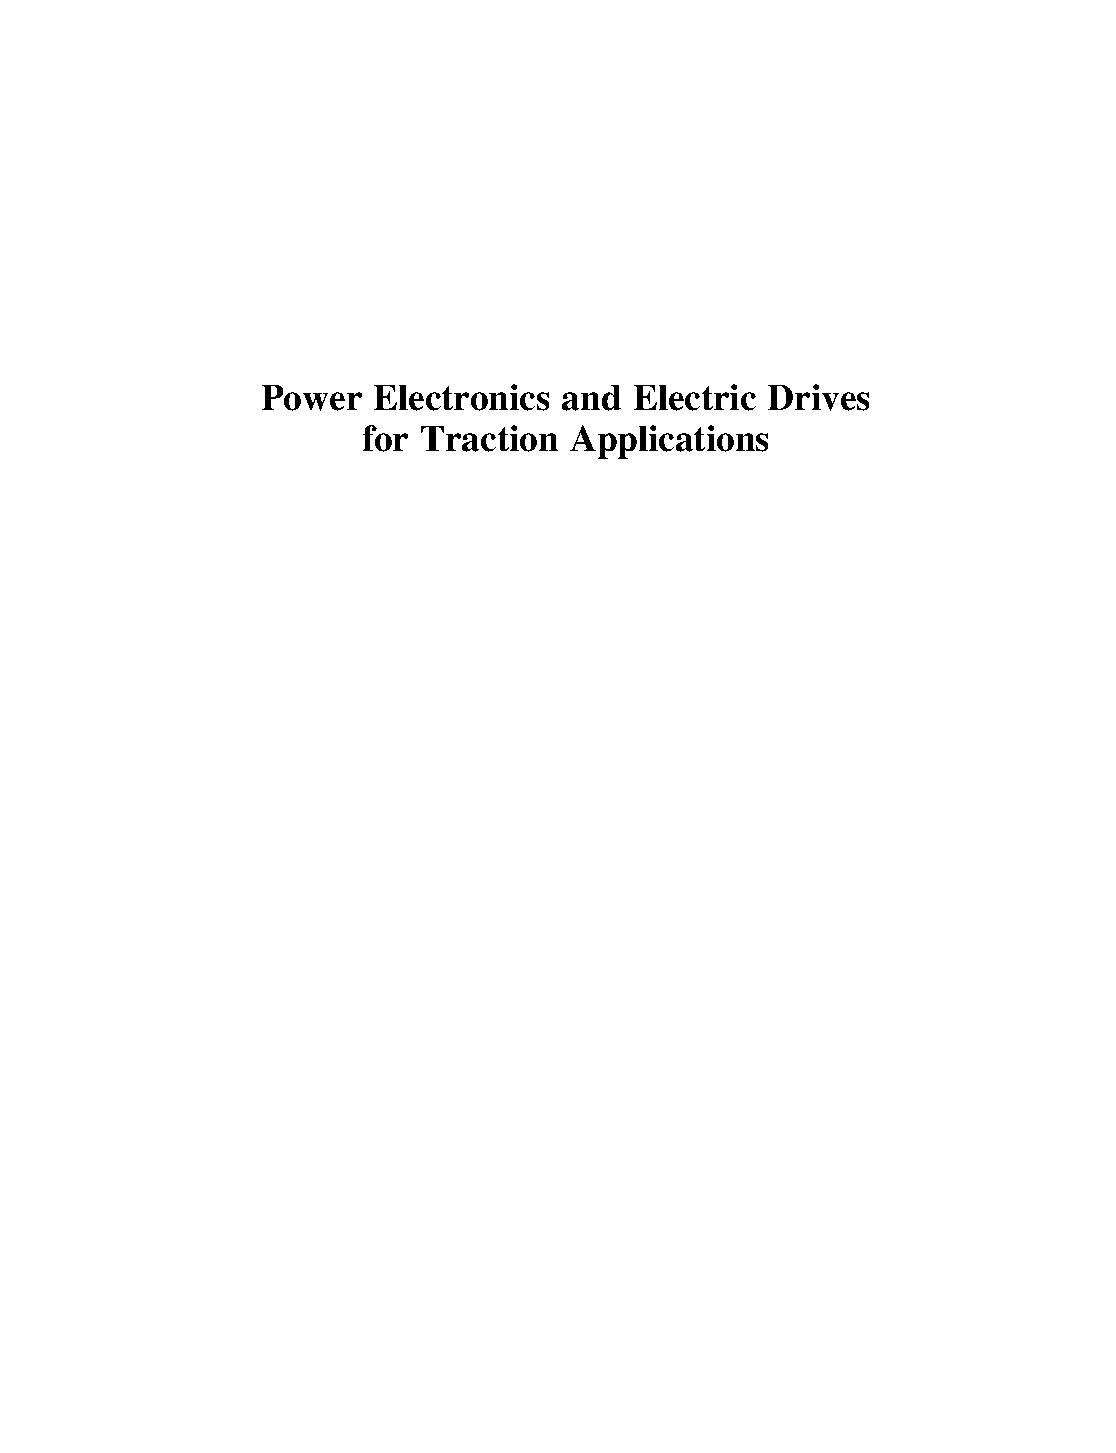
\includegraphics[width=0.7\textwidth,keepaspectratio]{figures/31.PowerS/abad2016}
	\caption{Railway main-line power supply systems in Europe. Adapted from \cite{abad2016}.}
	\label{fig:abad2016}
\end{figure}



\subsection{Railway power supply system}

Similarly to the electrical grid where a broad area of loads must be supplied, the railway power system must be capable of maintaining trains running in a broad area. The energy is supplied to the railway system through traction substations, similarly to the generation units of the electrical grid.

These traction substations ensure the interface between the electrical grid and the railway system, being responsible of supplying the distribution line of the railway system - or catenary.

As previously referred, the catenary can be divided in three main topologies:

%\begin{itemize}
%	\setlength\itemsep{-0.5em}
%	
%	\item DC supply system (six-, or 12-pulse diode rectifiers);
%	
%	\item AC 50Hz (or 60Hz) supply system;
%	
%	\item AC 16.7Hz supply system;
%
%\end{itemize}

\paragraph{1. DC supply system\\}

The DC supply system depends on rectifier converters (controlled or uncontrolled) as illustrated in figure \ref{fig:abad2016b}. This railway power supply topology requires several traction substations, towards the reduction of power losses in catenary due to the high value of current. In figure \ref{fig:abad2016f} is presented the supply architecture of such lines.

\paragraph{2. AC 50Hz (or 60Hz) supply system\\}

With AC catenaries, low frequency single-phase transformer is required to step down the catenary voltage (25 kV or 15 kV) to the rectifier operating voltage (the rectifier is a single-phase voltage source converter, usually with bi-directional power flow).

On the traction substation, a special setup of power transformers avoids the usage of complete power converters. In figure \ref{fig:abad2016d} is presented the substation setup to supply a single-phase 50Hz catenary.

\subsubsection{3. AC 16.7Hz supply systems\\}
An alternative setup is presented in figure \ref{fig:abad2016e} where a single-phase 16.7Hz supply voltage is generated with a complete power converter. 
%\vspace{-2.5em}
\begin{figure}[h!]
	\centering
	\begin{minipage}{.45\textwidth}
		\centering
%		\vspace{2.5em}
		\includegraphics[width=\textwidth,keepaspectratio]{figures/31.PowerS/abad2016b}
%		\vspace{2em}
		\captionof{figure}{6-pulse and 12-pulse diode rectifier configurations. Adapted from \cite{abad2016}.}
		\label{fig:abad2016b}
	\end{minipage}%
	\begin{minipage}{.03\textwidth}  ~\end{minipage}	
	\begin{minipage}{.375\textwidth}
		\centering
		\includegraphics[width=\textwidth,keepaspectratio]{figures/31.PowerS/abad2016f}
%		\vspace{0.5em}
		\captionof{figure}{DC supply system architecture. Adapted from \cite{abad2016}.}
		\label{fig:abad2016f}
	\end{minipage}
\end{figure}


\begin{figure}[h!]
	\centering
	\begin{minipage}{.45\textwidth}
		\centering
		%		\vspace{2.5em}
		\includegraphics[width=\textwidth,keepaspectratio]{figures/31.PowerS/abad2016d}
		%		\vspace{2em}
		\captionof{figure}{6-pulse and 12-pulse diode rectifier configurations. Adapted from \cite{abad2016}.}
		\label{fig:abad2016d}
	\end{minipage}%
	\begin{minipage}{.03\textwidth}  ~\end{minipage}	
	\begin{minipage}{.375\textwidth}
		\centering
		\includegraphics[width=\textwidth,keepaspectratio]{figures/31.PowerS/abad2016e}
		%		\vspace{0.5em}
		\captionof{figure}{DC supply system architecture. Adapted from \cite{abad2016}.}
		\label{fig:abad2016e}
	\end{minipage}
\end{figure}












\begin{figure}[h!]
	\centering
	\includegraphics[width=0.7\textwidth,keepaspectratio]{figures/31.PowerS/abad2016c}
	\caption{Railway main-line power supply systems in Europe. Adapted from \cite{abad2016}.}
	\label{fig:abad2016c}
\end{figure}

\begin{figure}[h!]
	\centering
	\includegraphics[width=0.7\textwidth,keepaspectratio]{figures/31.PowerS/abad2016g}
	\caption{Railway main-line power supply systems in Europe. Adapted from \cite{abad2016}.}
	\label{fig:abad2016g}
\end{figure}


\subsection{Traction substation transformer overview}

\subsection{Train power transformer}

\subsection{Train motor and power converter}

\subsection{Auxiliary loads}